\documentclass[
11pt, % The default document font size, options: 10pt, 11pt, 12pt
%codirector, % Uncomment to add a codirector to the title page
]{charter} 


% El títulos de la memoria, se usa en la carátula y se puede usar el cualquier lugar del documento con el comando \ttitle
\titulo{Optimización biomecánica del ciclismo asistida por inteligencia artificial
} 

% Nombre del posgrado, se usa en la carátula y se puede usar el cualquier lugar del documento con el comando \degreename
%\posgrado{Carrera de Especialización en Sistemas Embebidos} 
%\posgrado{Carrera de Especialización en Internet de las Cosas} 
\posgrado{Carrera de Especialización en Inteligencia Artificial}
%\posgrado{Maestría en Sistemas Embebidos} 
%\posgrado{Maestría en Internet de las cosas}

% Tu nombre, se puede usar el cualquier lugar del documento con el comando \authorname
% IMPORTANTE: no omitir titulaciones ni tildación en los nombres, también se recomienda escribir los nombres completos (tal cual los tienen en su documento)
\autor{Ing. Rodrigo Iván Goñi}

% El nombre del director y co-director, se puede usar el cualquier lugar del documento con el comando \supname y \cosupname y \pertesupname y \pertecosupname
\director{MSc. Fernado Corteggiano}
\pertenenciaDirector{FNRC} 
\codirector{} % para que aparezca en la portada se debe descomentar la opción codirector en los parámetros de documentclass
\pertenenciaCoDirector{FIUBA}

% Nombre del cliente, quien va a aprobar los resultados del proyecto, se puede usar con el comando \clientename y \empclientename
\cliente{Nombre del cliente}
\empresaCliente{Empresa del cliente}
 
\fechaINICIO{24 de junio de 2025}		%Fecha de inicio de la cursada de GdP \fechaInicioName
\fechaFINALPlan{16 de agosto de 2025} 	%Fecha de final de cursada de GdP
\fechaFINALTrabajo{15 de mayo de 2026}	%Fecha de defensa pública del trabajo final


\begin{document}

\maketitle
\thispagestyle{empty}
\pagebreak


\thispagestyle{empty}
{\setlength{\parskip}{0pt}
\tableofcontents{}
}
\pagebreak


\section*{Registros de cambios}
\label{sec:registro}


\begin{table}[ht]
\label{tab:registro}
\centering
\begin{tabularx}{\linewidth}{@{}|c|X|c|@{}}
\hline
\rowcolor[HTML]{C0C0C0} 
Revisión & \multicolumn{1}{c|}{\cellcolor[HTML]{C0C0C0}Detalles de los cambios realizados} & Fecha      \\ \hline
0      & Creación del documento                                 &\fechaInicioName \\ \hline
1      & Se completa hasta el punto 5 inclusive                & 07 de julio de 2025 \\ \hline
2      & Se completa hasta el punto 9 inclusive					 & 15 de julio de 2025 \\ \hline
3      & Se completa hasta el punto 12 inclusive					 & 29 de julio de 2025 \\ \hline
%		  Se puede agregar algo más \newline
%		  En distintas líneas \newline
%		  Así                                                    & {día} de {mes} de 202X \\ \hline
%3      & Se completa hasta el punto 12 inclusive                & {día} de {mes} de 202X \\ \hline
%4      & Se completa el plan	                                 & {día} de {mes} de 202X \\ \hline

% Si hay más correcciones pasada la versión 4 también se deben especificar acá

\end{tabularx}
\end{table}

\pagebreak



\section*{Acta de constitución del proyecto}
\label{sec:acta}

\begin{flushright}
Buenos Aires, \fechaInicioName
\end{flushright}

\vspace{2cm}

Por medio de la presente se acuerda con el \authorname\hspace{1px} que su Trabajo Final de la \degreename\hspace{1px} se titulará ``\ttitle'' y consistirá en el desarrollo de un prototipo de un sistema inteligente que, mediante la integración de la detección de pose por redes neuronales y el análisis de datos de sensores, optimice los parámetros biomecánicos de la bicicleta para maximizar la potencia, eficiencia y minimizar el riesgo de lesiones del ciclista. El trabajo tendrá un presupuesto preliminar estimado de 600 horas y un costo estimado de \$15000, con fecha de inicio el \fechaInicioName\hspace{1px} y fecha de presentación pública el \fechaFinalName.

Se adjunta a esta acta la planificación inicial.

\vfill

% Esta parte se construye sola con la información que hayan cargado en el preámbulo del documento y no debe modificarla
\begin{table}[ht]
\centering
\begin{tabular}{ccc}
\begin{tabular}[c]{@{}c@{}}Dr. Ing. Ariel Lutenberg \\ Director posgrado FIUBA\end{tabular} & \hspace{2cm} & \begin{tabular}[c]{@{}c@{}}\clientename \\ \empclientename \end{tabular} \vspace{2.5cm} \\ 
\multicolumn{3}{c}{\begin{tabular}[c]{@{}c@{}} \supname \\ Director del Trabajo Final\end{tabular}} \vspace{2.5cm} \\
\end{tabular}
\end{table}




\section{1. Descripción técnica-conceptual del proyecto a realizar}
\label{sec:descripcion}
La biomecánica en el ciclismo es un factor fundamental para mejorar el rendimiento y prevenir lesiones. Se basa en el principio de adaptar la bicicleta a las características físicas del ciclista. Un ajuste incorrecto no solo puede causar lesiones, sino también disminuir la potencia de salida hasta en un 20\%. Sin embargo, el acceso a un análisis biomecánico profesional presenta barreras significativas: las soluciones actuales suelen ser costosas, de baja disponibilidad y requieren visitas a laboratorios especializados.

El desafío principal de este proyecto es encontrar el balance óptimo entre la posición que maximiza la velocidad y aquella que minimiza el esfuerzo y el riesgo de lesiones. Frecuentemente, la postura más aerodinámica no es la más sostenible a largo plazo. Para abordar este problema, se propone el desarrollo de un sistema que ajuste automáticamente los parámetros de la bicicleta. Mediante el uso de inteligencia artificial, el sistema analizará la postura del ciclista para optimizar la potencia de salida y reducir la tensión muscular, lo que exige un enfoque de optimización multiobjetivo con diversas restricciones.

Las soluciones convencionales se basan en un análisis estático y puntual, realizado en un único día y dependiente en gran medida de la experiencia del biomecánico. La recomendación de repetir el ajuste anualmente, sumada a su alto costo y escasa disponibilidad, provoca que la mayoría de los ciclistas no mantengan una configuración óptima en sus bicicletas.

El valor fundamental de este sistema radica en ofrecer al ciclista la capacidad de realizar autoajustes frecuentes, de forma autónoma y a un costo significativamente menor que las alternativas tradicionales. Esto democratiza el acceso a una biomecánica de precisión, lo que permite una mejora continua del rendimiento y la prevención de lesiones.

Para lograr estos objetivos, el sistema propuesto se estructura en una serie de módulos interconectados, como se ilustra en el diagrama de bloques de la figura \ref{fig:diagBloques} a continuación:

\begin{figure}[htpb]
\centering
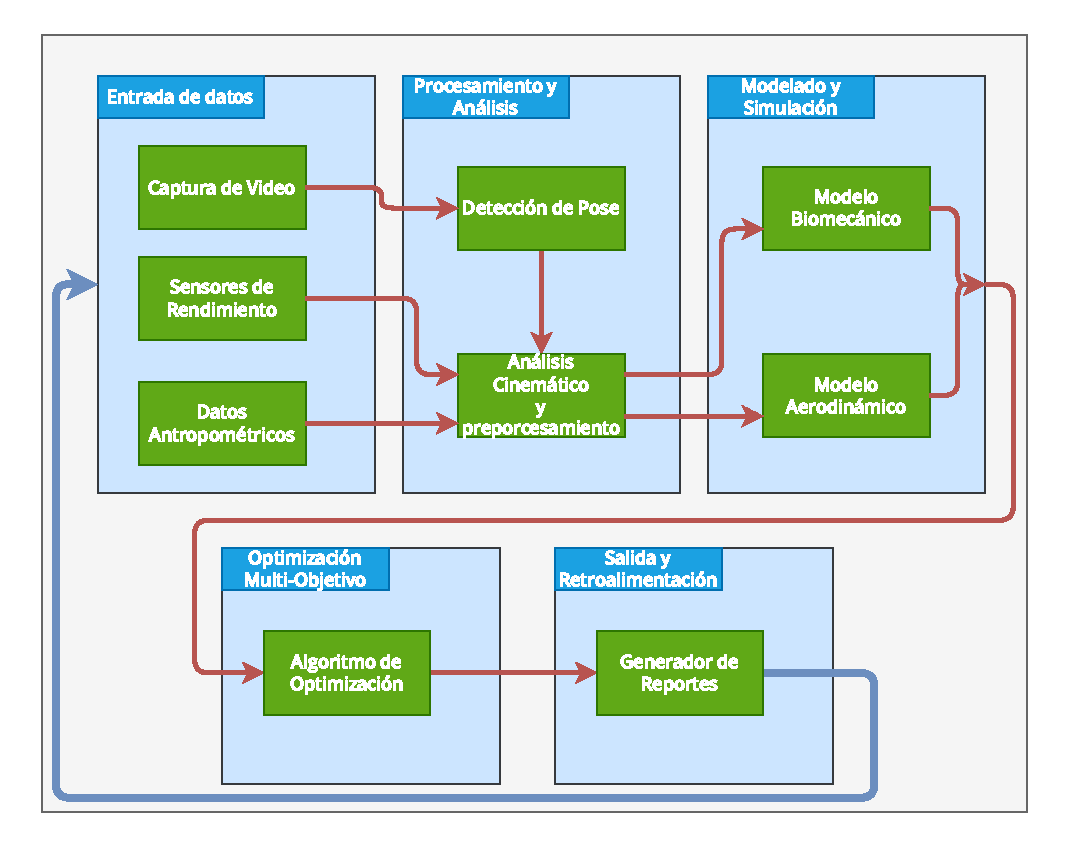
\includegraphics[width=.65\textwidth]{./Figuras/Diagrama_de_Bloques_proyecto_ciclista.pdf}
\caption{Diagrama en bloques del sistema.}
\label{fig:diagBloques}
\end{figure}

\begin{itemize}
\item Entrada de datos: este módulo es el encargado de recolectar datos de las distintas fuentes de información. Se compone de una fuente de video, sensores de rendimiento y los datos antropomórficos del ciclista.
\item Procesamiento y análisis: este módulo toma los datos de entrada y los procesa. Con la ayuda de una red neuronal de detección de pose, añade los datos de posición del ciclista al sistema. Luego, en un módulo de preprocesamiento, los datos se filtran, sincronizan, limpian y completan.
\item Modelado y simulación: con ayuda de un modelo físico y aerodinámico, se predice cómo impactarán los cambios de los parámetros de la bicicleta en el rendimiento.
\item Optimización multi-objetivo: con un algoritmo genético, se buscará maximizar la performance del objetivo en un rango adecuado de posición, tratando de minimizar la resistencia aerodinámica y teniendo en cuenta la morfología y el nivel del ciclista.
\item Salida y retroalimentación: con los datos de la optimización, se generará un reporte de recomendaciones y posibles configuraciones de la bicicleta. Una vez finalizado el reporte, se recomienda ajustar los parámetros para volver a iniciar el análisis.
\end{itemize}




\section{2. Identificación y análisis de los interesados}
\label{sec:interesados}


\begin{table}[ht]
%\caption{Identificación de los interesados}
%\label{tab:interesados}
\begin{tabularx}{\linewidth}{@{}|l|X|X|l|@{}}
\hline
\rowcolor[HTML]{C0C0C0} 
Rol           & Nombre y Apellido & Organización 	& Puesto 	\\ \hline
Responsable   & \authorname       & FIUBA        	& Alumno 	\\ \hline
Orientador    & \supname	      & \pertesupname 	& Director del Trabajo Final \\ \hline
Usuario final &          Ciclistas de distintos tipos         &        -      	&     -   	\\ \hline
\end{tabularx}
\end{table}

\begin{itemize}

\item Responsable: cl \authorname  es el líder del proyecto de optimización biomecánica asistida por IA. Es ingeniero en mecatrónica.

\item Orientador: cl \supname	, ingeniero electricista y magister en ciencias de la ingeniería de la UNRC, es director y profesor adjunto. Ya ha dirigido diversas tesis, aportará su experiencia en electrónica, telecomunicaciones y software, para definir el alcance y requerimientos del sistema.
\item Usuario final: ciclistas de distintos tipos que buscan optimizar la comodidad o el rendimiento de su bicicleta a través de ajustes personalizados.
\end{itemize}



\section{3. Propósito del proyecto}
\label{sec:proposito}
El propósito de este proyecto es desarrollar un sistema inteligente y personalizado que, mediante la integración de la detección de pose por redes neuronales y el análisis exhaustivo de datos provenientes de sensores de ciclismo, optimice los parámetros biomecánicos de la bicicleta. Esto incluye la altura y posición del sillín, la longitud de las bielas, la altura y ancho del manillar. El objetivo principal es maximizar la potencia y eficiencia del pedaleo, minimizar el riesgo de lesiones y equilibrar estos factores con la aerodinámica.
Este sistema permitirá a los ciclistas realizar autoajustes frecuentes, de forma autónoma y a un costo significativamente menor que las alternativas tradicionales, lo que democratiza el acceso a una biomecánica de precisión y permite una mejora continua del rendimiento y la prevención de lesiones.

\section{4. Alcance del proyecto}
\label{sec:alcance}

El proyecto incluye:
\begin{itemize}
\item Desarrollo de un sistema de optimización personalizado: proporcionará recomendaciones para el ajuste biomecánico de la bicicleta, que busquen maximizar el rendimiento (medido por la potencia y velocidad), la eficiencia y prevenir lesiones.

\item Ciclo continuo de análisis y retroalimentación: el sistema funcionará a través de las siguientes etapas:
    \begin{itemize}
        \item Captura de datos:
            \begin{itemize}
             	\item Calibración de la cámara.
                \item Grabación de videos del ciclista pedaleando.
                \item Recopilación simultánea de datos de rendimiento mediante sensores de potencia, cadencia y velocidad.
            \end{itemize}
        \item Análisis y modelado:
            \begin{itemize}
                \item Análisis de movimiento: uso de red neuronal de estimación de pose para extraer coordenadas 2D de puntos clave del cuerpo del ciclista desde los videos.
                \item Análisis cinemático: estudio de ángulos de articulaciones, fluidez del pedaleo y variabilidad del movimiento.
                \item Modelo biomecánico: creación de un modelo digital del sistema ciclista y bicicleta para simular el impacto de los ajustes en la potencia y el riesgo de lesión.
            \end{itemize}
        \item Optimización integral: un algoritmo de optimización analizará combinaciones para lograr el equilibrio perfecto entre:
            \begin{itemize}
                \item Ajuste biomecánico: determinación de la configuración óptima de componentes.
                \item Aerodinámica: evaluación de la postura del ciclista para la resistencia del aire, que buscará la posición más aerodinámica y sostenible.
                \item Prevención de lesiones: penalización de configuraciones que aumenten el estrés en articulaciones.
            \end{itemize}
        \item Recomendación y re-evaluación: generación de un reporte con recomendaciones claras para ajustar la bicicleta, que permita nuevas sesiones de captura de datos para refinar el ajuste.
    \end{itemize}

\item Adquisición y uso de datos:
    \begin{itemize}
        \item Videos de ciclismo grabados desde el lateral y el frontal.
        \item Datos de sensores sincronizados: potencia, cadencia y velocidad.
        \item Datos antropométricos del ciclista y configuración actual de la bicicleta.
        \item Utilización de recursos propios y entorno controlado para pruebas sistemáticas y sincronización precisa.
    \end{itemize}
\end{itemize}

El presente proyecto no incluye:
\begin{itemize}
\item El desarrollo de hardware personalizado para la captura de datos, más allá de la integración con sensores comerciales existentes.
\item El entrenamiento de la red neuronal de detección de pose desde cero. se espera utilizar o adaptar redes neuronales preexistentes.
\item La integración con todos los posibles modelos de bicicletas y componentes del mercado.
\item La simulación de factores externos complejos como condiciones climáticas extremas o interacciones con el tráfico.
\end{itemize}

\section{5. Supuestos del proyecto}
\label{sec:supuestos}

Para el desarrollo del presente proyecto se supone que:
\begin{itemize}
\item Se dispondrá de un rodillo de entrenamiento inteligente y sus respectivos sensores (potenciómetro, cadencia, velocidad) para la captura de datos en un entorno controlado y la realización de pruebas sistemáticas.
\item Se tendrá acceso a una cámara de video con capacidad para grabar en alta resolución.
\item La red neuronal de detección de pose (como Keypoint R-CNN o MediaPipe) a utilizar será lo suficientemente robusta y precisa para extraer los puntos clave del cuerpo del ciclista necesarios para el análisis biomecánico, y que su rendimiento será adecuado para el procesamiento de video.
\item Existirá suficiente disponibilidad de datos propios y de la comunidad.
\item El entorno de desarrollo y las herramientas de software necesarias son adecuadas.
\item Se contará con el tiempo y los recursos humanos necesarios para la investigación, desarrollo, implementación y realización de pruebas del sistema, incluida la mano de obra propia para la ejecución del proyecto.
\item Se contará con la revisión y retroalimentación constante del director del proyecto, \supname	, para asegurar la correcta orientación técnica y académica.
\item Las condiciones de iluminación durante la captura de video serán adecuadas para permitir una detección de pose precisa.
\item El proyecto se centrará en optimizaciones biomecánicas para el ciclismo en carretera o interior en rodillo.
\item Las variaciones individuales en la anatomía y flexibilidad de los ciclistas podrán ser adecuadamente modeladas y tenidas en cuenta por el algoritmo de optimización.
\end{itemize}

\section{6. Product Backlog}
\label{sec:backlog}

\begin{itemize}
  \item Épica 1: adquisición y preprocesamiento de datos biomecánicos.
    \begin{itemize}
      \item HU1: como ciclista, quiero que el sistema tome mi imagen de pedaleo para analizar mi postura.
        \begin{itemize}
          \item Dificultad: 3
          \item Complejidad: 2
          \item Incertidumbre: 2
          \item Suma: 7 $\rightarrow$ Story points: 8
        \end{itemize}
      \item HU2: como ingeniero, quiero consolidar un proceso de obtención de datos coordinado y automatizado para asegurar la eficiencia del análisis.
        \begin{itemize}
          \item Dificultad: 4
          \item Complejidad: 4
          \item Incertidumbre: 3
          \item Suma: 11 $\rightarrow$ Story points: 13
        \end{itemize}
      \item HU3: como ingeniero en inteligencia artificial, quiero aplicar técnicas de visión por computadora para obtener automáticamente los puntos clave de mi cuerpo en los videos de pedaleo, de manera que el análisis biomecánico sea preciso.
        \begin{itemize}
          \item Dificultad: 5
          \item Complejidad: 5
          \item Incertidumbre: 4
          \item Suma: 14 $\rightarrow$ Story points: 21
        \end{itemize}
      \item HU4: como científico de datos, quiero realizar un análisis exploratorio de los datos y filtrarlos correctamente para asegurar la calidad de la información utilizada en los modelos.
        \begin{itemize}
          \item Dificultad: 3
          \item Complejidad: 3
          \item Incertidumbre: 2
          \item Suma: 8 $\rightarrow$ Story points: 8
        \end{itemize}
    \end{itemize}
  \item Épica 2: modelado y optimización biomecánica.
    \begin{itemize}
      \item HU5: como ingeniero de software, quiero que el sistema simule las condiciones de pedaleo y el impacto de los ajustes mecánicos para predecir los resultados de la optimización.
        \begin{itemize}
          \item Dificultad: 4
          \item Complejidad: 4
          \item Incertidumbre: 3
          \item Suma: 11 $\rightarrow$ Story points: 13
        \end{itemize}
      \item HU6: como ingeniero, necesito modelar un algoritmo de optimización biomecánica multi-objetivo para encontrar la configuración de bicicleta más eficiente y cómoda.
        \begin{itemize}
          \item Dificultad: 5
          \item Complejidad: 5
          \item Incertidumbre: 5
          \item Suma: 15 $\rightarrow$ Story points: 21
        \end{itemize}
      \item HU7: Como ingeniero, necesito un sistema de optimización que considere la morfología y el nivel del ciclista para ofrecer recomendaciones personalizadas y efectivas.
        \begin{itemize}
          \item Dificultad: 4
          \item Complejidad: 3
          \item Incertidumbre: 3
          \item Suma: 10 $\rightarrow$ Story points: 13
        \end{itemize}
    \end{itemize}
  \item Épica 3: generación de recomendaciones y experiencia de usuario.
    \begin{itemize}
      \item HU8: como ciclista, quiero recibir un reporte claro y conciso con las recomendaciones de configuración de mi bicicleta para poder realizar los ajustes yo mismo.
        \begin{itemize}
          \item Dificultad: 3
          \item Complejidad: 3
          \item Incertidumbre: 2
          \item Suma: 8 $\rightarrow$ Story points: 8
        \end{itemize}
      \item HU9: como usuario, quiero que la interfaz me permita ingresar fácilmente los parámetros relevantes del ciclista y la bicicleta para obtener un análisis preciso.
        \begin{itemize}
          \item Dificultad: 3
          \item Complejidad: 2
          \item Incertidumbre: 2
          \item Suma: 7 $\rightarrow$ Story points: 8
        \end{itemize}
    \end{itemize}
  \item Épica 4: validación y mejora continua del sistema.
    \begin{itemize}
      \item HU10: como ciclista, quiero poder re-evaluar mi postura y rendimiento después de aplicar los ajustes recomendados para refinar la optimización.
        \begin{itemize}
          \item Dificultad: 3
          \item Complejidad: 2
          \item Incertidumbre: 2
          \item Suma: 7 $\rightarrow$ Story points: 8
        \end{itemize}
      \item HU11: como desarrollador, necesito un entorno controlado para realizar pruebas sistemáticas y asegurar la precisión del sistema.
        \begin{itemize}
          \item Dificultad: 4
          \item Complejidad: 3
          \item Incertidumbre: 3
          \item Suma: 10 $\rightarrow$ Story points: 13
        \end{itemize}
    \end{itemize}
\end{itemize}


\section{7. Criterios de aceptación de historias de usuario}
\label{sec:criteriosAceptacion}

\begin{itemize}
  \item Épica 1: adquisición y preprocesamiento de datos biomecánicos.
    \begin{itemize}
      \item Criterios de aceptación HU1:
        \begin{itemize}
          \item El sistema debe activar y controlar la cámara de manera autónoma para la captura de video del ciclista mientras pedalea.
          \item El ciclista debe recibir una confirmación visual o sonora clara de que la grabación ha comenzado y finalizado correctamente.
          \item Los videos capturados deben guardarse automáticamente en un formato específico.
        \end{itemize}
      \item Criterios de aceptación HU2:
        \begin{itemize}
          \item Tras la subida de un video, el sistema debe iniciar automáticamente la secuencia de preprocesamiento y extracción de datos.
          \item El ingeniero debe poder visualizar el progreso de la obtención y procesamiento de los datos en una interfaz de estado.
          \item El sistema debe registrar un log detallado de cada paso del proceso de obtención de datos, que incluya la hora de inicio y fin, y cualquier error.
        \end{itemize}
      \item Criterios de aceptación HU3:
        \begin{itemize}
          \item El algoritmo debe identificar correctamente los puntos clave del esqueleto del ciclista en cada fotograma del video.
          \item Los puntos clave detectados deben superponerse visualmente sobre el video original para una verificación rápida de la precisión por parte del ingeniero.
          \item La tasa de detección de puntos clave debe ser adecuada y en un tiempo razonable.
        \end{itemize}
      \item Criterios de aceptación HU4:
        \begin{itemize}
          \item El sistema debe permitir la aplicación de filtros predefinidos a los datos de los puntos clave.
          \item Se deben generar gráficos de distribución y series temporales para cada punto clave y métrica, que permitan la identificación visual de anomalías.
          \item La aplicación de filtros debe reducir el ruido en los datos al menos en un 20\% sin perder información relevante, según métricas preestablecidas.
        \end{itemize}
    \end{itemize}
  \item Épica 2: modelado y optimización biomecánica.
    \begin{itemize}
      \item Criterios de aceptación HU5:
        \begin{itemize}
          \item El sistema debe ser capaz de simular las métricas biomecánicas clave para configuraciones de bicicleta diferentes.
          \item Los resultados de la simulación deben presentarse en gráficos comparativos que muestren claramente el impacto de cada ajuste en las métricas.
          \item Cada simulación individual debe completarse en un tiempo adecuado.
        \end{itemize}
      \item Criterios de aceptación HU6:
        \begin{itemize}
          \item El algoritmo debe generar un conjunto de soluciones de Pareto que maximicen la eficiencia, minimicen la incomodidad y respeten las restricciones biomecánicas.
          \item Las soluciones del frente de Pareto deben visualizarse en un gráfico que permita al ingeniero entender el balance entre los diferentes objetivos.
          \item El algoritmo debe demostrar convergencia hacia un conjunto de soluciones estables y diversas dentro de un número razonable de generaciones o iteraciones.
        \end{itemize}
      \item Criterios de aceptación HU7:
        \begin{itemize}
          \item El sistema debe ajustar los rangos de optimización y las ponderaciones de los objetivos con base en los datos de morfología y nivel del ciclista.
          \item Las recomendaciones generadas deben mostrar una justificación clara de cómo la morfología y el nivel del ciclista influyeron en los ajustes sugeridos.
          \item Los modelos internos deben integrar los parámetros morfológicos y de nivel del ciclista como variables de entrada en el proceso de optimización.
        \end{itemize}
    \end{itemize}
  \item Épica 3: generación de recomendaciones y experiencia de usuario.
    \begin{itemize}
      \item Criterios de aceptación HU8:
        \begin{itemize}
          \item El sistema debe generar un reporte descargable que incluya las configuraciones de la bicicleta recomendadas.
          \item El reporte debe contener diagramas o imágenes que ilustren visualmente cada ajuste y su ubicación en la bicicleta.
          \item El reporte debe ser compatible con lectores de PDF estándar y poder ser accedido desde dispositivos móviles y de escritorio.
        \end{itemize}
      \item Criterios de aceptación HU9:
        \begin{itemize}
          \item La interfaz debe presentar campos de entrada de datos claros y con etiquetas descriptivas para todos los parámetros requeridos.
          \item La interfaz debe ofrecer validación en tiempo real de los datos ingresados e indicar errores de formato o rangos inválidos de forma intuitiva.
          \item La interfaz debe ser compatible con los navegadores web modernos.
        \end{itemize}
    \end{itemize}
  \item Épica 4: validación y mejora continua del sistema.
    \begin{itemize}
      \item Criterios de aceptación HU10:
        \begin{itemize}
          \item El sistema debe permitir al ciclista iniciar un nuevo ciclo de captura de video y análisis de postura para una reevaluación.
          \item El sistema debe generar un informe comparativo que visualice los cambios en la postura y las métricas de rendimiento entre la evaluación inicial y la reevaluación.
          \item Los datos de cada reevaluación deben almacenarse, vincularse con el historial del ciclista y permitir el acceso a versiones anteriores.
        \end{itemize}
      \item Criterios de aceptación HU11:
        \begin{itemize}
          \item El entorno debe permitir la ejecución de pruebas unitarias, de integración y de extremo a extremo para todas las funcionalidades principales del sistema.
          \item Los resultados de las pruebas deben visualizarse en un dashboard o reporte que muestre el estado de las pruebas de forma clara.
          \item El entorno de pruebas debe ser reproducible y configurable para simular diferentes entornos y conjuntos de datos.
        \end{itemize}
    \end{itemize}
\end{itemize}

\section{8. Fases de CRISP-DM}
\label{sec:crisp}

A continuación se detallan las fases del modelo CRISP-DM aplicadas al proyecto.

\begin{enumerate}
  \item Comprensión del negocio:
    \begin{itemize}
      \item Objetivo: el proyecto busca desarrollar un prototipo de sistema inteligente que optimice los parámetros biomecánicos de una bicicleta. El propósito principal es maximizar la potencia y eficiencia del pedaleo, mientras se minimiza el riesgo de lesiones y se equilibra con la aerodinámica para alcanzar la máxima velocidad posible.
      \item Valor agregado de IA: la inteligencia artificial se utilizará para analizar la postura del ciclista a través de redes neuronales de detección de pose y para ejecutar un algoritmo de optimización multiobjetivo.
      \item Métricas de éxito: el éxito del proyecto se medirá por la capacidad del sistema para generar un reporte con recomendaciones claras y cuantificables. Además, la mejora en el rendimiento y la comodidad del ciclista se verificará a través de métricas objetivas y subjetivas post-ajuste, lo que permite un ciclo de reevaluación para validar el impacto positivo de las sugerencias.
    \end{itemize}

  \item Comprensión de los datos:
    \begin{itemize}
      \item Tipo y origen:
        \begin{itemize}
          \item Videos del ciclista: grabaciones desde perspectivas lateral y frontal para el análisis de pose.
          \item Datos de sensores: información de rendimiento como potencia (W), cadencia (RPM) ritmo cardíaco (BPM), y velocidad (km/h), recopilada de forma simultánea a los videos.
          \item Datos antropométricos: medidas del ciclista y de la configuración inicial de su bicicleta.
        \end{itemize}
      \item Cantidad y calidad: se utilizarán recursos propios, que incluyen un rodillo de entrenamiento inteligente que permite realizar pruebas en un entorno controlado. Esta configuración es clave para garantizar la sincronización precisa entre el video y los datos de los sensores. Para enriquecer el dataset, se podrán utilizar datos de plataformas comunitarias como Strava o Zwift.
    \end{itemize}

  \item Preparación de los datos:
    \begin{itemize}
      \item Características clave y transformaciones:
        \begin{itemize}
          \item Se aplicarán técnicas de visión por computadora, mediante una red neuronal de estimación de pose, como Keypoint R-CNN o MediaPipe, para extraer las coordenadas 2D de puntos clave del cuerpo del ciclista a partir de los videos.
          \item Los datos de sensores y los puntos clave extraídos serán filtrados, sincronizados, limpiados y completados en un módulo de preprocesamiento.
          \item A partir de las coordenadas, se realizará un análisis cinemático para estudiar ángulos de articulaciones, fluidez del pedaleo y variabilidad del movimiento.
        \end{itemize}
    \end{itemize}

  \item Modelado:
    \begin{itemize}
      \item Tipo de problema: el núcleo del proyecto es un problema de optimización multiobjetivo. Se busca encontrar el balance óptimo entre la aerodinámica y la potencia, ya que la postura más aerodinámica no siempre es la más potente o sostenible.
      \item Algoritmos posibles: se planea utilizar un algoritmo genético para explorar el espacio de soluciones y encontrar una configuración óptima de la bicicleta. Este algoritmo trabajará sobre un modelo físico que predice cómo los cambios en los parámetros impactan en el rendimiento. Además, se creará un modelo biomecánico digital para simular el efecto de los ajustes.
    \end{itemize}

  \item Evaluación del modelo:
\begin{itemize}
    \item Métricas de rendimiento: la evaluación no se centrará en métricas de clasificación tradicionales. En su lugar, se evaluará la calidad de las soluciones generadas por el algoritmo de optimización. El algoritmo deberá producir un conjunto de soluciones en el frente de Pareto que representen los mejores compromisos posibles entre los objetivos.
    \item Métricas cuantificables y automatizables:
    \begin{itemize}
        \item Reducción de la frecuencia cardíaca (FC) para una potencia dada: a una potencia de salida constante, un menor ritmo cardíaco post-ajuste indicaría una mayor eficiencia cardiovascular y un menor esfuerzo percibido. Esto es directamente medible con los sensores.
        \item Reducción de la variabilidad de ángulos críticos: una menor desviación estándar en ángulos articulares clave a lo largo del ciclo de pedaleo puede indicar mayor fluidez, estabilidad y menor riesgo de lesiones. Esto es automatizable a partir del análisis cinemático.
    \end{itemize}
    \item Métricas subjetivas (para validación funcional):
    \begin{itemize}
        \item Percepción del esfuerzo (RPE): el ciclista reporta su nivel de esfuerzo en una escala de 6 a 20 para una sesión de potencia y duración predefinida. Una disminución del RPE sería un indicador de confort y eficiencia.
        \item Escalas de dolor/molestia: reportes del ciclista sobre la ausencia o reducción de molestias en articulaciones o músculos específicos.
    \end{itemize}
    \item Proceso de evaluación: la validación final será funcional. El sistema generará un reporte con recomendaciones claras. El ciclista aplicará los ajustes y realizará una nueva sesión de captura de datos en el entorno controlado. En esta nueva sesión, se compararán las métricas objetivas y se recopilarán las métricas subjetivas con respecto a la configuración inicial. Esto permitirá cerrar un ciclo de mejora continua y validar empíricamente la efectividad de las recomendaciones.
\end{itemize}
\end{enumerate}

\section{9. Desglose del trabajo en tareas}
\label{sec:wbs}

\begin{longtable}{@{}|l|>{\raggedright\arraybackslash}p{0.5\linewidth}|c|c|@{}}

\caption{Desglose de tareas del proyecto} \label{tab:wbs} \\

\hline
\rowcolor[HTML]{C0C0C0}
Historia de usuario & Tarea técnica & Estimación & Prioridad \\
\hline
\endfirsthead

\multicolumn{4}{c}%
{{\tablename\ \thetable{} -- continuación de la página anterior}} \\
\hline
\rowcolor[HTML]{C0C0C0}
Historia de usuario & Tarea técnica & Estimación & Prioridad \\
\hline
\endhead

\hline \multicolumn{4}{r}{{Continúa en la página siguiente}} \\
\endfoot

\hline
\endlastfoot

% Contenido de la tabla
\multicolumn{4}{|l|}{Épica 1: adquisición y preprocesamiento de datos biomecánicos} \\ \hline
HU1 & Investigar y seleccionar la librería de Python para el control de la cámara. & 4 h & Alta \\ \hline
HU1 & Desarrollar el script para iniciar/detener la grabación y guardar el video. & 8 h & Alta \\ \hline
HU2 & Configurar la recolección de datos de sensores en sincronía con el video. & 8 h & Alta \\ \hline
HU2 & Implementar una función para la carga de datos antropométricos y de la bicicleta. & 6 h & Media \\ \hline
HU2 & Desarrollar el script que automatice la ejecución secuencial de la captura de video y sensores. & 8 h & Alta \\ \hline
HU3 & Investigar y comparar modelos pre-entrenados para la detección de pose. & 8 h & Alta \\ \hline
HU3 & Implementar el modelo seleccionado para procesar los videos y extraer coordenadas 2D de puntos clave. & 8 h & Alta \\ \hline
HU3 & Desarrollar una función para visualizar los puntos clave superpuestos en los fotogramas para verificación. & 6 h & Media \\ \hline
HU4 & Desarrollar scripts para la carga y visualización inicial de datos. & 8 h & Alta \\ \hline
HU4 & Implementar filtros para suavizar el ruido en los datos de sensores y coordenadas. & 8 h & Media \\ \hline
HU4 & Escribir funciones para detectar y gestionar valores atípicos o faltantes en las series de datos. & 6 h & Media \\ \hline
\multicolumn{4}{|l|}{Épica 2: modelado y optimización biomecánica} \\ \hline
HU5 & Desarrollar el modelo físico-matemático que relacione los ángulos articulares con la potencia y la eficiencia. & 8 h & Alta \\ \hline
HU5 & Implementar una función que reciba los parámetros de la bicicleta y simule el impacto en el modelo. & 8 h & Alta \\ \hline
HU5 & Crear visualizaciones para mostrar los resultados de la simulación. & 6 h & Media \\ \hline
HU6 & Investigar y seleccionar una librería de Python para algoritmos genéticos. & 8 h & Alta \\ \hline
HU6 & Definir la función de fitness multiobjetivo. & 8 h & Alta \\ \hline
HU6 & Implementar el algoritmo genético para que explore el espacio de soluciones y encuentre el frente de Pareto. & 8 h & Alta \\ \hline
HU7 & Definir cómo los datos de entrada ajustarán los rangos y pesos del optimizador. & 8 h & Alta \\ \hline
HU7 & Integrar las variables de personalización como parámetros de entrada en el modelo de simulación. & 8 h & Media \\ \hline
HU7 & Ajustar la función de fitness para que penalice soluciones no viables según el perfil del ciclista. & 8 h & Media \\ \hline
\multicolumn{4}{|l|}{Épica 3: generación de recomendaciones y experiencia de usuario} \\ \hline
HU8 & Diseñar la estructura y contenido del reporte final en PDF. & 6 h & Alta \\ \hline
HU8 & Desarrollar el script que genere el reporte en PDF con textos, datos y gráficos de forma automática. & 8 h & Alta \\ \hline
HU9 & Desarrollar una interfaz de usuario simple para la entrada de datos. & 8 h & Media \\ \hline
HU9 & Implementar validaciones de entrada para asegurar que los datos del usuario sean correctos y estén en rango. & 6 h & Baja \\ \hline
\multicolumn{4}{|l|}{Épica 4: validación y mejora continua del sistema} \\ \hline
HU10 & Implementar la funcionalidad para guardar y cargar sesiones de análisis previas. & 8 h & Media \\ \hline
HU10 & Desarrollar un módulo que genere un reporte comparativo entre dos sesiones de un mismo ciclista. & 8 h & Media \\ \hline
HU11 & Estructurar el proyecto para permitir pruebas unitarias de los módulos clave. & 8 h & Alta \\ \hline
HU11 & Crear un conjunto de datos de prueba para validar el pipeline completo. & 8 h & Media \\ \hline
HU11 & Escribir pruebas de integración que verifiquen la correcta comunicación entre los módulos del sistema. & 8 h & Media \\

\end{longtable}

\section{10. Planificación de Sprints}

\begin{longtable}{|l|l|p{0.4\linewidth}|c|l|c|}

\caption{Planificación detallada de sprints del proyecto}
\label{tab:sprints} \\

% --- ENCABEZADO PARA LA PRIMERA PÁGINA ---
\hline
\rowcolor[HTML]{C0C0C0}
Sprint & HU o Fase & Tarea técnica o de gestión & Horas & Responsable & \% comp. \\
\hline
\endfirsthead

% --- ENCABEZADO PARA LAS PÁGINAS SIGUIENTES ---
\multicolumn{6}{l}{\tablename\ \thetable{} -- continuación de la página anterior} \\
\hline
\rowcolor[HTML]{C0C0C0}
Sprint & HU o Fase & Tarea técnica o de gestión & Horas & Responsable & \% comp. \\
\hline
\endhead

% --- PIE DE PÁGINA PARA TODAS MENOS LA ÚLTIMA ---
\hline
\multicolumn{6}{r}{{continúa en la página siguiente}} \\
\endfoot

% --- PIE DE PÁGINA PARA LA ÚLTIMA PÁGINA ---
\hline
\multicolumn{3}{|r|}{Total de horas estimadas} & 600 h & & \\
\hline
\endlastfoot

% --- CONTENIDO DE LA TABLA ---

Sprint 0 & Planificación & Definición del alcance, cronograma y acta constitutiva. & 15 h & Alumno & 70\% \\
Sprint 0 & Planificación & Configuración del entorno de desarrollo y repositorios. & 10 h & Alumno & 80\% \\ \hline

Sprint 1 & HU1 & Investigación y selección de librería para control de cámara. & 8 h & Alumno & 50\% \\
Sprint 1 & HU1, HU2 & Desarrollo del script de grabación y sincronización de sensores. & 20 h & Alumno & 0\% \\
Sprint 1 & Gestión & Documentación continua del sprint. & 5 h & Alumno & 0\% \\ \hline

Sprint 2 & HU2 & Desarrollo del script para automatizar la captura de datos. & 18 h & Alumno & 0\% \\
Sprint 2 & HU3 & Investigación y comparación de modelos de estimación de pose. & 12 h & Alumno & 100\% \\
Sprint 2 & HU3 & Implementación de la extracción de puntos clave de videos. & 15 h & Alumno & 90\% \\
Sprint 2 & Gestión & Documentación continua del sprint. & 5 h & Alumno & 0\% \\ \hline

Sprint 3 & HU3 & Desarrollo de función para visualización del esqueleto. & 12 h & Alumno & 50\% \\
Sprint 3 & HU4 & Desarrollo de scripts para carga y análisis exploratorio (EDA). & 18 h & Alumno & 0\% \\
Sprint 3 & HU4 & Implementación de filtros para suavizado y limpieza de datos. & 15 h & Alumno & 0\% \\
Sprint 3 & Gestión & Documentación continua del sprint. & 5 h & Alumno & 0\% \\ \hline

Sprint 4 & HU5 & Desarrollo del modelo físico-matemático del ciclista. & 25 h & Alumno & 0\% \\
Sprint 4 & HU5 & Implementación de la simulación de ajustes posturales. & 20 h & Alumno & 0\% \\
Sprint 4 & Gestión & Documentación continua del sprint. & 5 h & Alumno & 0\% \\ \hline

Sprint 5 & HU6 & Investigación y selección de librería para optimización genética. & 10 h & Alumno & 0\% \\
Sprint 5 & HU6 & Definición de la función de fitness multiobjetivo. & 25 h & Alumno & 0\% \\
Sprint 5 & HU9 & Desarrollo de interfaz de usuario para la entrada de datos. & 15 h & Alumno & 0\% \\
Sprint 5 & Gestión & Documentación continua del sprint. & 5 h & Alumno & 0\% \\ \hline

Sprint 6 & HU6 & Implementación del algoritmo genético para la optimización. & 30 h & Alumno & 0\% \\
Sprint 6 & HU7 & Definición de la influencia de datos de entrada en el optimizador. & 15 h & Alumno & 0\% \\
Sprint 6 & Gestión & Documentación continua del sprint. & 5 h & Alumno & 0\% \\ \hline

Sprint 7 & HU7 & Integración de variables de personalización en el modelo. & 20 h & Alumno & 0\% \\
Sprint 7 & HU8 & Diseño de la estructura y plantilla del reporte en PDF. & 10 h & Alumno & 0\% \\
Sprint 7 & HU8 & Desarrollo del script para la generación automática del reporte. & 15 h & Alumno & 0\% \\
Sprint 7 & Gestión & Documentación continua del sprint. & 5 h & Alumno & 0\% \\ \hline

Sprint 8 & HU11 & Creación de un conjunto de datos de prueba con casos conocidos. & 20 h & Alumno & 0\% \\
Sprint 8 & HU11 & Escritura de pruebas de integración para el flujo completo. & 25 h & Alumno & 0\% \\
Sprint 8 & Gestión & Documentación continua del sprint. & 5 h & Alumno & 0\% \\ \hline

Sprint 9 & HU10 & Implementación de guardado y carga de sesiones de análisis. & 20 h & Alumno & 0\% \\
Sprint 9 & HU10 & Desarrollo de reporte comparativo entre sesiones. & 20 h & Alumno & 0\% \\
Sprint 9 & Gestión & Documentación continua del sprint. & 5 h & Alumno & 0\% \\ \hline

Sprint 10 & Memoria & Redacción de secciones iniciales e intermedias de la memoria. & 45 h & Alumno & 0\% \\
Sprint 10 & Gestión & Revisión y ajustes con tutor. & 5 h & Alumno & 0\% \\ \hline

Sprint 11 & Memoria & Redacción final y revisión completa de la memoria. & 25 h & Alumno & 0\% \\
Sprint 11 & Defensa & Preparación de la presentación y material de defensa. & 25 h & Alumno & 0\% \\

\end{longtable}

\section{11. Diagrama de Gantt (sprints)}
\label{sec:gantt_sprints}

Para mejorar la legibilidad del diagrama de Gantt, se utilizan identificadores abreviados para cada tarea. La siguiente tabla detalla la correspondencia entre cada ID y su descripción completa.

\begin{longtable}{|l|p{0.8\linewidth}|}
\caption{Tabla de referencias para las tareas del diagrama de Gantt.}
\label{tab:gantt_ref_sprints} \\
\hline
\rowcolor{gray}
\textbf{ID} & \textbf{Descripción de la tarea} \\
\hline
\endfirsthead
\multicolumn{2}{l}{\tablename\ \thetable{} -- continuación de la página anterior} \\
\hline
\rowcolor{gray}
\textbf{ID} & \textbf{Descripción de la tarea} \\
\hline
\endhead
\hline
\endfoot
\hline
\endlastfoot

% --- Sprint 0 ---
\multicolumn{2}{l}{\textbf{Sprint 0: planificación}} \\
S0.1 & Definición del alcance, cronograma y acta constitutiva \\
S0.2 & Configuración del entorno de desarrollo y repositorios \\ \hline
% --- Sprint 1 ---
\multicolumn{2}{l}{\textbf{Sprint 1: adquisición de datos (HU1, HU2)}} \\
S1.1 & Investigación y selección de librería para control de cámara \\
S1.2 & Desarrollo del script de grabación y sincronización de sensores \\
S1.3 & Documentación continua del sprint \\ \hline
% --- Sprint 2 ---
\multicolumn{2}{l}{\textbf{Sprint 2: preprocesamiento (HU2, HU3)}} \\
S2.1 & Desarrollo del script para automatizar la captura de datos \\
S2.2 & Investigación y comparación de modelos de estimación de pose \\
S2.3 & Implementación de la extracción de puntos clave de videos \\
S2.4 & Documentación continua del sprint \\ \hline
% --- Sprint 3 ---
\multicolumn{2}{l}{\textbf{Sprint 3: análisis y visualización (HU3, HU4)}} \\
S3.1 & Desarrollo de función para visualización del esqueleto \\
S3.2 & Desarrollo de scripts para carga y análisis exploratorio (EDA) \\
S3.3 & Implementación de filtros para suavizado y limpieza de datos \\
S3.4 & Documentación continua del sprint \\ \hline
% --- Sprint 4 ---
\multicolumn{2}{l}{\textbf{Sprint 4: modelado (HU5)}} \\
S4.1 & Desarrollo del modelo físico-matemático del ciclista \\
S4.2 & Implementación de la simulación de ajustes posturales \\
S4.3 & Documentación continua del sprint \\ \hline
% --- Sprint 5 ---
\multicolumn{2}{l}{\textbf{Sprint 5: optimización y ui (HU6, HU9)}} \\
S5.1 & Investigación y selección de librería para optimización genética \\
S5.2 & Definición de la función de fitness multiobjetivo \\
S5.3 & Desarrollo de interfaz de usuario para la entrada de datos \\
S5.4 & Documentación continua del sprint \\ \hline
% --- Sprint 6 ---
\multicolumn{2}{l}{\textbf{Sprint 6: implementación de optimización (HU6, HU7)}} \\
S6.1 & Implementación del algoritmo genético para la optimización \\
S6.2 & Definición de la influencia de datos de entrada en el optimizador \\
S6.3 & Documentación continua del sprint \\ \hline
% --- Sprint 7 ---
\multicolumn{2}{l}{\textbf{Sprint 7: personalización y reportes (HU7, HU8)}} \\
S7.1 & Integración de variables de personalización en el modelo \\
S7.2 & Diseño de la estructura y plantilla del reporte en PDF \\
S7.3 & Desarrollo del script para la generación automática del reporte \\
S7.4 & Documentación continua del sprint \\ \hline
% --- Sprint 8 ---
\multicolumn{2}{l}{\textbf{Sprint 8: pruebas (HU11)}} \\
S8.1 & Creación de un conjunto de datos de prueba con casos conocidos \\
S8.2 & Escritura de pruebas de integración para el flujo completo \\
S8.3 & Documentación continua del sprint \\ \hline
% --- Sprint 9 ---
\multicolumn{2}{l}{\textbf{Sprint 9: funcionalidades extra (HU10)}} \\
S9.1 & Implementación de guardado y carga de sesiones de análisis \\
S9.2 & Desarrollo de reporte comparativo entre sesiones \\
S9.3 & Documentación continua del sprint \\ \hline
% --- Sprint 10 ---
\multicolumn{2}{l}{\textbf{Sprint 10: redacción de memoria}} \\
S10.1 & Redacción de secciones iniciales e intermedias de la memoria \\
S10.2 & Revisión y ajustes con el tutor \\ \hline
% --- Sprint 11 ---
\multicolumn{2}{l}{\textbf{Sprint 11: cierre de proyecto}} \\
S11.1 & Redacción final y revisión completa de la memoria \\
S11.2 & Preparación de la presentación y material de defensa \\
\end{longtable}

\vspace{0.5cm}

\begin{ganttchart}[
    hgrid,
    vgrid,
    x unit=0.6cm, 
    y unit title=0.7cm,
    y unit chart=0.45cm,
    bar label node/.append style={align=left, font=\bfseries\scriptsize}, % ID de tarea en negrita
    group label node/.append style={align=left, font=\small\bfseries},
    bar height=0.6,
    group height=0.7,
    group/.append style={fill=groupgray},
    bar/.append style={fill=techblue},
    group top shift=0.1,
    bar top shift=0.2,
    title label font=\bfseries
  ]{1}{24}

\gantttitle{Cronograma del proyecto por sprints (semanas)}{24} \\
\gantttitlelist{1,...,24}{1}

% Los títulos de grupo y las etiquetas de barra ahora están corregidos y abreviados.
\ganttgroup{Sprint 0}{1}{2} \\
\ganttbar[bar/.append style={fill=nontechgreen}]{S0.1}{1}{2} \\
\ganttbar[bar/.append style={fill=nontechgreen}]{S0.2}{1}{2} \\

\ganttgroup{Sprint 1}{3}{4} \\
\ganttbar{S1.1}{3}{3} \\
\ganttbar{S1.2}{3}{4} \\
\ganttbar[bar/.append style={fill=nontechgreen}]{S1.3}{3}{4} \\

\ganttgroup{Sprint 2}{5}{6} \\
\ganttbar{S2.1}{5}{6} \\
\ganttbar{S2.2}{5}{5} \\
\ganttbar{S2.3}{6}{6} \\
\ganttbar[bar/.append style={fill=nontechgreen}]{S2.4}{5}{6} \\

\ganttgroup{Sprint 3}{7}{8} \\
\ganttbar{S3.1}{7}{7} \\
\ganttbar{S3.2}{7}{8} \\
\ganttbar{S3.3}{8}{8} \\
\ganttbar[bar/.append style={fill=nontechgreen}]{S3.4}{7}{8} \\

\ganttgroup{Sprint 4}{9}{10} \\
\ganttbar{S4.1}{9}{10} \\
\ganttbar{S4.2}{9}{10} \\
\ganttbar[bar/.append style={fill=nontechgreen}]{S4.3}{9}{10} \\

\ganttgroup{Sprint 5}{11}{12} \\
\ganttbar{S5.1}{11}{11} \\
\ganttbar{S5.2}{11}{12} \\
\ganttbar{S5.3}{12}{12} \\
\ganttbar[bar/.append style={fill=nontechgreen}]{S5.4}{11}{12} \\

\ganttgroup{Sprint 6}{13}{14} \\
\ganttbar{S6.1}{13}{14} \\
\ganttbar{S6.2}{13}{14} \\
\ganttbar[bar/.append style={fill=nontechgreen}]{S6.3}{13}{14} \\

\ganttgroup{Sprint 7}{15}{16} \\
\ganttbar{S7.1}{15}{16} \\
\ganttbar{S7.2}{15}{15} \\
\ganttbar{S7.3}{16}{16} \\
\ganttbar[bar/.append style={fill=nontechgreen}]{S7.4}{15}{16} \\

\ganttgroup{Sprint 8}{17}{18} \\
\ganttbar{S8.1}{17}{18} \\
\ganttbar{S8.2}{17}{18} \\
\ganttbar[bar/.append style={fill=nontechgreen}]{S8.3}{17}{18} \\

\ganttgroup{Sprint 9}{19}{20} \\
\ganttbar{S9.1}{19}{20} \\
\ganttbar{S9.2}{19}{20} \\
\ganttbar[bar/.append style={fill=nontechgreen}]{S9.3}{19}{20} \\

\ganttgroup{Sprint 10}{21}{22} \\
\ganttbar[bar/.append style={fill=nontechgreen}]{S10.1}{21}{22} \\
\ganttbar[bar/.append style={fill=nontechgreen}]{S10.2}{21}{22} \\

\ganttgroup{Sprint 11}{23}{24} \\
\ganttbar[bar/.append style={fill=nontechgreen}]{S11.1}{23}{24} \\
\ganttbar[bar/.append style={fill=nontechgreen}]{S11.2}{23}{24} \\

\ganttmilestone[milestone/.append style={fill=red}]{E.F.}{24}
\end{ganttchart}

\section{12. Normativa y cumplimiento de datos (gobernanza)}

El proyecto gestiona datos personales y sensibles, por lo que su tratamiento exige el cumplimiento estricto de la normativa vigente. Los datos que se recolectan incluyen:
\begin{itemize}
    \item Datos personales: videos con la imagen del ciclista, sus medidas antropométricas y las métricas de rendimiento (potencia, cadencia) que se asocian a él.
    \item Datos sensibles: la frecuencia cardíaca (FC), por ser un dato relativo a la salud y requerir un nivel superior de protección.
\end{itemize}

El marco legal principal es la ley 25.326 de Protección de Datos Personales de la República Argentina, y se adoptan como referencia los principios del Reglamento General de Protección de Datos (RGPD) europeo. Para garantizar la legalidad y la ética del proyecto, se establecen los siguientes requisitos obligatorios:
\begin{itemize}
    \item Consentimiento explícito: se debe obtener el consentimiento informado de cada ciclista antes de la recolección de datos, con un detalle claro de la finalidad del tratamiento y los derechos del titular.
    \item Limitación de la finalidad: el uso de los datos se restringe exclusivamente al objetivo del proyecto, que es la optimización biomecánica.
    \item Seguridad y confidencialidad: es imperativa la implementación de medidas técnicas para la protección de los datos. Se prioriza la anonimización en las etapas tempranas del proceso para mitigar riesgos.
\end{itemize}

En conclusión, el proyecto es viable desde el punto de vista legal y ético. Su ejecución se condiciona a la correcta y continua aplicación del marco de gobernanza de datos aquí descrito. Al centrarse en el uso de recursos propios en un entorno controlado, el proyecto tiene una gran ventaja para implementar correctamente estos controles.


Aquí tienes el código LaTeX completo para tu sección de gestión de riesgos. Puedes copiarlo y pegarlo directamente en tu editor TeXmaker.

Para que el código funcione correctamente, asegúrate de tener los siguientes paquetes cargados en el preámbulo de tu documento:


\section{13. Gestión de riesgos}
\label{sec:riesgos}

\subsection*{a) Identificación de los riesgos y estimación de sus consecuencias}

\subsubsection*{Riesgo 1: Complejidad técnica subestimada y desvío del alcance (scope creep)}

El proyecto integra múltiples disciplinas complejas (visión por computadora, biomecánica, optimización con algoritmos genéticos y desarrollo de software). Existe el riesgo de que la interconexión de estos módulos o la dificultad de uno de ellos sea mayor a la estimada, lo que puede causar retrasos significativos o una expansión no controlada del alcance original.
\begin{itemize}
  \item Severidad (s): 8.\\
  Justificación: Si la complejidad se subestima, podría ser imposible completar funcionalidades clave del sistema (como el módulo de optimización) dentro del cronograma académico. Esto comprometería directamente la entrega del producto final y el cumplimiento de los objetivos centrales del proyecto.
  \item Probabilidad de ocurrencia (o): 7.\\
  Justificación: A pesar de contar con 4 años de experiencia, la naturaleza del proyecto es inherentemente investigativa y multidisciplinaria. Para un solo desarrollador, la probabilidad de encontrar obstáculos técnicos imprevistos en al menos una de las áreas es alta.
\end{itemize}   

\subsubsection*{Riesgo 2: Calidad y sincronización de datos deficiente}

El núcleo del sistema depende de la recolección simultánea y precisa de datos de video, potencia, cadencia y frecuencia cardíaca. Un fallo en la sincronización temporal o la captura de datos de baja calidad (por ejemplo, videos con mala iluminación o sensores que se desconectan) invalida por completo los resultados del análisis.
\begin{itemize}
  \item Severidad (s): 9.\\
  Justificación: Este riesgo es crítico. Si los datos de entrada son incorrectos ("basura entra, basura sale"), el modelo biomecánico y el optimizador generarán recomendaciones inútiles o, en el peor de los casos, perjudiciales para el ciclista. Esto invalida la premisa fundamental del proyecto.
  \item Probabilidad de ocurrencia (o): 6.\\
  Justificación: La probabilidad es moderadamente alta. Aunque se usará un entorno controlado, la tarea de asegurar una sincronización perfecta a nivel de milisegundos entre una cámara y múltiples sensores (usualmente Bluetooth/ANT+) es un desafío técnico conocido y propenso a fallos intermitentes.
\end{itemize}

\subsubsection*{Riesgo 3: Inexactitud del modelo de detección de pose preentrenado}

El proyecto asume que un modelo preentrenado (como MediaPipe o Keypoint R-CNN) será suficientemente preciso para identificar los puntos articulares del ciclista. Si el modelo no tiene el rendimiento esperado en el contexto específico del ciclismo (vistas laterales, oclusiones parciales, movimiento rápido), el análisis cinemático será erróneo.
\begin{itemize}
  \item Severidad (s): 8.\\
  Justificación: La precisión de las coordenadas 2D de las articulaciones es la base para todo el cálculo de ángulos y el modelado biomecánico. Un error en esta etapa se propagaría y amplificaría en todo el sistema, lo que lleva a conclusiones y recomendaciones incorrectas.
  \item Probabilidad de ocurrencia (o): 5.\\
  Justificación: La probabilidad es media. Los modelos modernos son muy robustos, pero no fueron entrenados exclusivamente para el análisis biomecánico de ciclistas. Factores como la ropa holgada, ángulos de cámara no ideales o condiciones de luz variables pueden degradar su precisión de forma inesperada.
\end{itemize}

\subsubsection*{Riesgo 4: Dependencia de una única persona (key person risk)}

El proyecto es desarrollado en su totalidad por una sola persona. Cualquier imprevisto personal, enfermedad, problema técnico bloqueante o incluso agotamiento (burnout) detendría por completo el progreso del proyecto, ya que no hay otro miembro del equipo que pueda continuar con las tareas.
\begin{itemize}
    \item Severidad (s): 10.\\
    Justificación: La severidad es máxima. La continuidad del proyecto depende al 100\% de la disponibilidad y capacidad del único desarrollador. No existe un plan de contingencia humano para su reemplazo.
    \item Probabilidad de ocurrencia (o): 4.\\
    Justificación: Se asume que el desarrollador está comprometido y sano. Sin embargo, en un proyecto de varios meses, la probabilidad de que surja algún imprevisto personal o un periodo de agotamiento no es despreciable, por lo que se asigna una probabilidad baja-moderada.
\end{itemize}

\subsubsection*{Riesgo 5: Dificultad para validar objetivamente las recomendaciones}

El proyecto tiene como objetivo mejorar el rendimiento y el confort, pero la validación de esta mejora es intrínsecamente difícil. Las métricas objetivas (como la FC a una potencia dada) pueden verse afectadas por muchos factores externos (fatiga, temperatura, estado de ánimo), y las métricas subjetivas (como la percepción del esfuerzo) son difíciles de cuantificar.
\begin{itemize}
    \item Severidad (s): 7.\\
    Justificación: Si no se puede demostrar con un grado razonable de certeza que las recomendaciones del sistema son efectivas, el proyecto pierde gran parte de su valor práctico y queda en un plano puramente teórico, lo que afectaría de forma negativa su evaluación final.
    \item Probabilidad de ocurrencia (o): 6.\\
    Justificación: La probabilidad de encontrar dificultades en la validación es moderadamente alta. Es un desafío conocido en la biomecánica deportiva el aislamiento del efecto de un solo cambio (el ajuste de la bicicleta) de todas las demás variables que influyen en el rendimiento de un atleta.
\end{itemize}


\subsection*{b) Tabla de gestión de riesgos}

\begin{table}[htpb]
\centering
\caption{Tabla de gestión de riesgos}
\label{tab:riesgos}
\begin{tabularx}{\linewidth}{@{}|X|c|c|c|c|c|c|@{}}
\hline
\rowcolor[HTML]{C0C0C0} 
Riesgo & S & O & RPN & S* & O* & RPN* \\ \hline
1. Complejidad técnica y scope creep & 8 & 7 & 56 & 8 & 4 & 32 \\ \hline
2. Calidad y sincronización de datos & 9 & 6 & 54 & 9 & 2 & 18 \\ \hline
3. Inexactitud del modelo de pose & 8 & 5 & 40 & 5 & 3 & 15 \\ \hline
4. Dependencia de una única persona & 10 & 4 & 40 & 7 & 4 & 28 \\ \hline
5. Dificultad en la validación & 7 & 6 & 42 & 5 & 4 & 20 \\ \hline
\end{tabularx}%
\end{table}

Criterio adoptado:

Se tomarán medidas de mitigación en los riesgos cuyos números de RPN iniciales sean mayores a 35. Según este criterio, todos los riesgos identificados requieren un plan de mitigación.

\vspace{0.5cm}

\subsection*{c) Plan de mitigación de los riesgos que originalmente excedían el RPN máximo establecido}
 
\subsubsection*{Riesgo 1: Complejidad técnica y "scope creep"}
\begin{itemize}
    \item Plan de mitigación:
    \begin{enumerate}
      \item Priorización del MVP (Producto Mínimo Viable): Enfocar los primeros sprints en el desarrollo de un \textit{pipeline} completo pero simple: captura de video y datos de sensores, procesamiento con el modelo de pose, aplicación de un modelo de optimización básico y generación de un reporte simple.
      \item Gestión estricta del alcance: Seguir de forma rigurosa el \textit{product backlog} definido. Cualquier nueva idea o mejora se registrará, pero no se implementará hasta que el MVP sea funcional.
      \item Reuniones de seguimiento semanales: Realizar reuniones obligatorias con el director del proyecto para la revisión del progreso, la discusión de bloqueos y la garantía de que el proyecto no se desvíe de los objetivos definidos.
    \end{enumerate}
  \item Nueva asignación de s* y o*, con su respectiva justificación:
  \begin{itemize}
  \item Severidad (s*): 8. La severidad intrínseca del riesgo no cambia, ya que el proyecto sigue con su complejidad.
  \item Probabilidad de ocurrencia (o*): 4. La probabilidad de que el riesgo impacte de forma negativa se reduce de manera significativa. La priorización del MVP asegura una entrega funcional y las reuniones con el supervisor actúan como un mecanismo de control para evitar el \textit{scope creep}.
  \end{itemize}
\end{itemize}

\subsubsection*{Riesgo 2: Calidad y sincronización de datos deficiente}
\begin{itemize}
    \item Plan de mitigación:
    \begin{enumerate}
        \item Protocolo de captura estandarizado: Definir y documentar un protocolo estricto para la toma de datos: posición fija de la cámara, uso de la misma iluminación artificial, vestimenta ajustada y de color sólido para el ciclista.
        \item Script de validación de sincronización: Desarrollar un script específico (como parte de HU2) que capture una ráfaga corta de datos y video, y genere un gráfico para la verificación visual de la alineación de los picos de potencia con el movimiento de pedaleo en el video. Este script se ejecutará antes de cada sesión de grabación principal.
        \item Módulo de chequeo automático: Implementar funciones en el preprocesamiento (HU4) que alerten automáticamente sobre datos faltantes, valores atípicos o desincronizaciones evidentes.
    \end{enumerate}
    \item Nueva asignación de s* y o*, con su respectiva justificación:
    \begin{itemize}
        \item Severidad (s*): 9. La severidad se mantiene. Datos de mala calidad aún serían catastróficos.
        \item Probabilidad de ocurrencia (o*): 2. La probabilidad se reduce de forma drástica. El protocolo y la validación previa a la captura minimizan la posibilidad de recolectar datos inutilizables, lo que transforma un riesgo probable en uno muy poco probable.
    \end{itemize}
\end{itemize}

\subsubsection*{Riesgo 3: Inexactitud del modelo de detección de pose preentrenado}
\begin{itemize}
    \item Plan de mitigación:
    \begin{enumerate}
        \item Evaluación comparativa: En la fase inicial (HU3), investigar y probar al menos dos modelos de pose distintos (ej. MediaPipe BlazePose, OpenPose) con videos propios para determinar cuál ofrece mayor precisión y estabilidad en un entorno de ciclismo.
        \item Visualización para verificación: Priorizar el desarrollo de la función que superpone el esqueleto detectado sobre el video. Esto permitirá una verificación visual rápida y constante de la calidad de la detección en cada etapa del desarrollo.
        \item Contingencia de "fine-tuning": Como plan de contingencia, si la precisión no es suficiente, se contempla la posibilidad de un \textit{fine-tuning} del modelo elegido sobre un pequeño set de imágenes de ciclistas con etiquetado manual.
    \end{enumerate}
    \item Nueva asignación de s* y o*, con su respectiva justificación:
    \begin{itemize}
        \item Severidad (s*): 5. La severidad se reduce. Al tener un plan de contingencia claro (prueba de otro modelo o reentrenamiento), el riesgo deja de ser un posible bloqueante total del proyecto y se convierte en un problema técnico con solución, aunque implique más trabajo.
        \item Probabilidad de ocurrencia (o*): 3. La probabilidad de que un modelo impreciso arruine el proyecto disminuye, ya que el plan de mitigación aborda el problema de frente mediante la evaluación y la preparación para una solución alternativa.
    \end{itemize}
\end{itemize}

\subsubsection*{Riesgo 4: Dependencia de una única persona (key person risk)}
\begin{itemize}
    \item Plan de mitigación:
    \begin{enumerate}
        \item Documentación y control de versiones riguroso: Mantener toda la documentación, código y resultados en un repositorio de Git (GitHub/GitLab) con \textit{commits} frecuentes y descriptivos. El proyecto ya cuenta con una documentación muy detallada (WBS, Sprints) que se debe mantener actualizada.
        \item Transferencia de conocimiento al supervisor: En las reuniones semanales, no solo reportar el estado, sino también explicar la arquitectura del código y las decisiones de diseño. Esto asegura que el director de carrera tenga un conocimiento suficiente para orientar o incluso auditar el código si fuera necesario.
        \item Planificación sostenible: Distribuir la carga de trabajo de manera realista a lo largo de los sprints para evitar el agotamiento, con la inclusión de semanas de "colchón" o para tareas de refactorización.
    \end{enumerate}
    \item Nueva asignación de s* y o*, con su respectiva justificación:
    \begin{itemize}
        \item Severidad (s*): 7. La severidad se reduce. Aunque una ausencia prolongada aún sería muy grave, la documentación y el conocimiento del supervisor harían el proyecto recuperable y no una pérdida total.
        \item Probabilidad de ocurrencia (o*): 4. La probabilidad del evento externo no cambia, pero se reduce la probabilidad de interrupción por causas controlables como el \textit{burnout}.
    \end{itemize}
\end{itemize}

\subsubsection*{Riesgo 5: Dificultad para validar objetivamente las recomendaciones}
\begin{itemize}
    \item Plan de mitigación:
    \begin{enumerate}
        \item Protocolo de validación A/B controlado: Definir un protocolo de prueba estricto: realizar una sesión de medición con la configuración inicial (A), aplicar los ajustes recomendados, permitir un breve periodo de adaptación, y realizar una segunda sesión idéntica (B). Ambas sesiones deben tener la misma duración y perfil de potencia en el rodillo.
        \item Métricas combinadas: No depender de una sola métrica. Evaluar el éxito con la combinación de la reducción de la FC a potencia constante, la reducción de la variabilidad de ángulos clave (obtenido del análisis cinemático) y un cuestionario estructurado de confort/dolor (escala de 1 a 10 para rodillas, espalda, hombros).
        \item Aceptación de la limitación: Reconocer explícitamente las limitaciones de la validación en la memoria final del proyecto y presentar los resultados como evidencia indicativa de la efectividad del modelo, en lugar de una prueba absoluta.
    \end{enumerate}
    \item Nueva asignación de s* y o*, con su respectiva justificación:
    \begin{itemize}
        \item Severidad (s*): 5. La severidad se reduce. Con la gestión de expectativas y un método de validación robusto (aunque no perfecto), un resultado no concluyente no significa el fracaso del proyecto, sino un hallazgo para analizar.
        \item Probabilidad de ocurrencia (o*): 4. La probabilidad de no poder validar nada se reduce. Un protocolo estructurado y el uso de métricas combinadas aumentan la probabilidad de detectar una señal positiva y obtener una conclusión significativa.
    \end{itemize}
\end{itemize}

\section{14. Sprint Review}
\label{sec:sprint_review}

La revisión de sprint (\emph{Sprint Review}) es una práctica fundamental en metodologías ágiles. Consiste en revisar y evaluar lo que se ha completado al finalizar un sprint. En esta instancia, se presentan los avances y se verifica si las funcionalidades cumplen con los criterios de aceptación establecidos. También se identifican entregables parciales y se consideran ajustes si es necesario.

Aunque el proyecto aún se encuentre en etapa de planificación, esta sección permite proyectar cómo se evaluarán las funcionalidades más importantes del backlog. Esta mirada anticipada favorece la planificación enfocada en valor y permite reflexionar sobre posibles obstáculos.

\textbf{Objetivo:} anticipar cómo se evaluará el avance del proyecto a medida que se desarrollen las funcionalidades, utilizando como base al menos cuatro historias de usuario del \emph{Product Backlog}.


Seleccionar al menos 4 HU del Product Backlog. Para cada una, completar la siguiente tabla de revisión proyectada:

\textbf{Formato sugerido:}
\begin{table}[htpb]
\renewcommand{\arraystretch}{1.5}
\begin{tabular}{|>{\raggedright\arraybackslash}m{2.5cm}|
                >{\raggedright\arraybackslash}m{2.3cm}|
                >{\raggedright\arraybackslash}m{3cm}|
                >{\raggedright\arraybackslash}m{3cm}|
                >{\raggedright\arraybackslash}m{3cm}|}
\hline
\rowcolor[HTML]{CCCCCC}
\textbf{HU seleccionada} & \textbf{Tareas asociadas} & \textbf{Entregable esperado} & \textbf{¿Cómo sabrás que está cumplida?} & \textbf{Observaciones o riesgos} \\
\hline
                         & Tarea 1 &                             &                                           &                                     \\ \cline{2-2}
\multirow{-2}{=}{HU1}    & Tarea 2 & \multirow{-2}{=}{Módulo funcional} & \multirow{-2}{=}{Cumple criterios de aceptación definidos} & \multirow{-2}{=}{Falta validar con el tutor} \\
\hline
                         & Tarea 1 &                             &                                           &                                     \\ \cline{2-2}
\multirow{-2}{=}{HU3}    & Tarea 2 & \multirow{-2}{=}{Reporte generado} & \multirow{-2}{=}{Exportación disponible y clara} & \multirow{-2}{=}{Requiere datos reales} \\
\hline
                         & Tarea 1 &                             &                                           &                                     \\ \cline{2-2}
\multirow{-2}{=}{HU5}    & Tarea 2 & \multirow{-2}{=}{Panel de gestión} & \multirow{-2}{=}{Roles diferenciados operativos} & \multirow{-2}{=}{Riesgo en integración} \\
\hline
                         & Tarea 1 &                             &                                           &                                     \\ \cline{2-2}
\multirow{-2}{=}{HU7}    & Tarea 2 & \multirow{-2}{=}{Informe trimestral} & \multirow{-2}{=}{PDF con gráficos y evolución} & \multirow{-2}{=}{Puede faltar tiempo para ajustes} \\
\hline
\end{tabular}
\end{table}

\section{15. Sprint Retrospective}    
\label{sec:sprint_retro}

La retrospectiva de sprint es una práctica orientada a la mejora continua. Al finalizar un sprint, el equipo (o el alumno, si trabaja de forma individual) reflexiona sobre lo que funcionó bien, lo que puede mejorarse y qué acciones concretas pueden implementarse para trabajar mejor en el futuro.

Durante la cursada se propuso el uso de la \textbf{Estrella de la Retrospectiva}, que organiza la reflexión en torno a cinco ejes:

\begin{itemize}
\item  ¿Qué hacer más?
\item  ¿Qué hacer menos?
\item  ¿Qué mantener?
\item  ¿Qué empezar a hacer?
\item  ¿Qué dejar de hacer?
\end{itemize}

Aun en una etapa temprana, esta herramienta permite que el alumno planifique su forma de trabajar, identifique anticipadamente posibles dificultades y diseñe estrategias de organización personal.

\textbf{Objetivo:} reflexionar sobre las condiciones iniciales del proyecto, identificando fortalezas, posibles dificultades y estrategias de mejora, incluso antes del inicio del desarrollo.


Completar la siguiente tabla tomando como referencia los cinco ejes de la Estrella de la Retrospectiva (\emph{Starfish} o estrella de mar). Esta instancia te ayudará a definir buenas prácticas desde el inicio y prepararte para enfrentar el trabajo de forma organizada y flexible. Se deberá completar la tabla al menos para 3 sprints técnicos y 1 no técnico.

\textbf{Formato sugerido:}

\begin{table}[htpb]
\renewcommand{\arraystretch}{1.4}
\begin{tabular}{|>{\raggedright\arraybackslash}p{1.8cm}|
                >{\raggedright\arraybackslash}p{2.3cm}|
                >{\raggedright\arraybackslash}p{2.3cm}|
                >{\raggedright\arraybackslash}p{2.3cm}|
                >{\raggedright\arraybackslash}p{2.3cm}|
                >{\raggedright\arraybackslash}p{2.3cm}|}
\hline
\rowcolor[HTML]{CCCCCC} 
\textbf{Sprint tipo y N°} & \textbf{¿Qué hacer más?} & \textbf{¿Qué hacer menos?} & \textbf{¿Qué mantener?} & \textbf{¿Qué empezar a hacer?} & \textbf{¿Qué dejar de hacer?} \\
\hline
Sprint técnico - 1 & Validaciones continuas con el alumno & Cambios sin versión registrada & Pruebas con datos simulados & Documentar cambios propuestos & Ajustes sin análisis de impacto \\
\hline
Sprint técnico - 2 & Verificar configuraciones en múltiples escenarios & Modificar parámetros sin guardar historial & Perfiles reutilizables & Usar logs para configuración & Repetir pruebas manuales innecesarias \\
\hline
Sprint técnico - 8 & Comparar correlaciones con casos previos & Cambiar parámetros sin justificar & Revisión cruzada de métricas & Anotar configuraciones usadas & Trabajar sin respaldo de datos \\
\hline
Sprint no técnico - 12 (por ej.: ``Defensa'') & Ensayos orales con feedback & Cambiar contenidos en la memoria & Material visual claro & Dividir la presentación por bloques & Agregar gráficos difíciles de explicar \\
\hline
\end{tabular}
\end{table}




\end{document}